\section{ОБЗОР ЛИТЕРАТУРЫ}
\label{sec:domain}

\subsection{Основные типы сообщений стандарта \iecStd-8-1}

Стандарт \iecStd\ описывает свод правил для организации событийного протокола
передачи данных. Область применения стандарта -- системы связи внутри подстанции.
В набор стандартов входят стандарт по одноранговой связи и связи клиент/сервер,
стандарт по структуре и конфигурации подстанции, стандарт по методике испытаний,
стандарт экологических требований и другие~\cite{iec_description}.

\begin{figure}[ht]
    \centering
    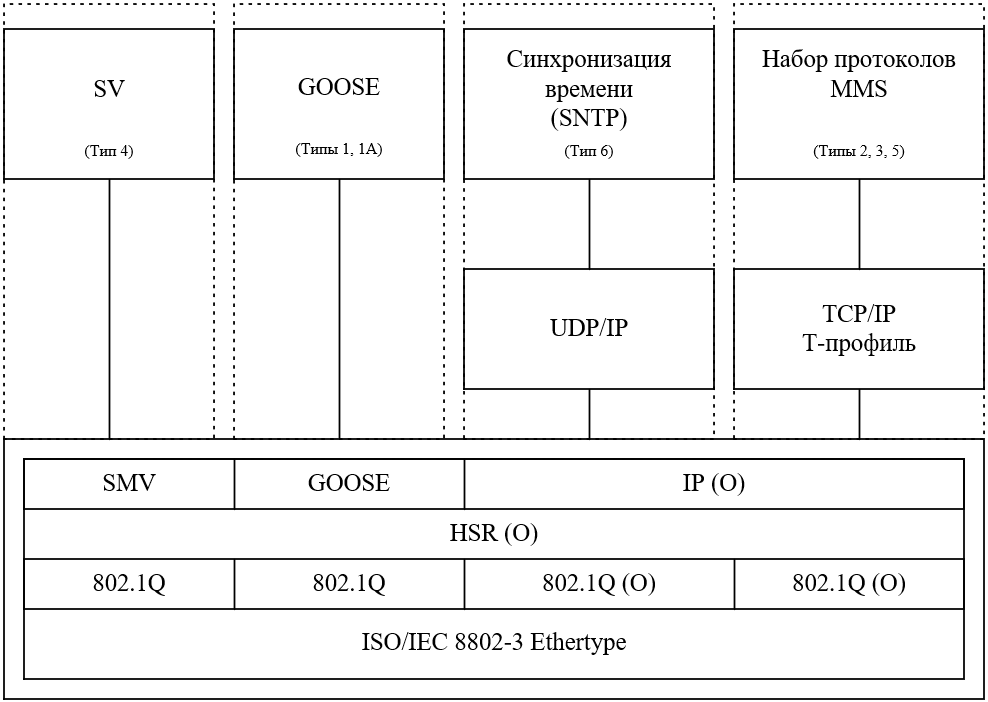
\includegraphics[width=1.0\linewidth]{msgTypes}
    \caption{Основные протоколы \iecStd}
    \label{pic::domain::msg_types}
\end{figure}

Целью стандарта \iecStdRef81\ является предоставление подробных
инструкций и
спецификаций в отношении механизмов и правил, необходимых для реализации сервисов,
объектов и алгоритмов, указанных в других стандартах \iec, таких как
\iecStd-7-2, \iecStd-7-3 и \iecStd-7-4~\cite{IEC61850_7_2, IEC61850_7_3,
IEC61850_7_4}, с использованием спецификаций производственных сообщений,
SNTP и других прикладных протоколов, как показано
на рисунке~\ref{pic::domain::msg_types}.
В стандарте описаны следующие типы сообщений:

\begin{itemize}
    \item тип 1 -- быстрые сообщения;
    \item тип 1А -- сообщения отключения;
    \item тип 2 -- сообщения со средней скоростью;
    \item тип 3 -- сообщения с низкой скоростью;
    \item тип 4 -- сообщения с необработанными данными;
    \item тип 5 -- функции передачи файлов;
    \item тип 6 -- сообщения синхронизации времени.
\end{itemize}

\nomenclaturex{SNTP}{Simple Network Time Protocol}{упрощенная реализация протокола синхронизации времени NTP}

Сообщения типов 1 и 1A сопоставляются с различными типами EtherType
(поле в кадре Ethernet) для оптимизации декодирования полученных сообщений.

\subsection{Соответствие с моделью OSI}

\nomenclaturex{OSI}{Open Systems Interconnection}{взаимосвязь открытых систем}

Эталонная модель OSI детализирует модель, основанную на концепции многоуровневой
коммуникационной функциональности. Модель конкретизирует семь уровней и выделяет
функциональные требования для каждого уровня, чтобы создать надежную систему связи.
Она не определяет протоколы, которые должны использоваться для достижения
функциональности, и не ограничивает решение одним набором протоколов.

\begin{figure}[ht]
    \centering
    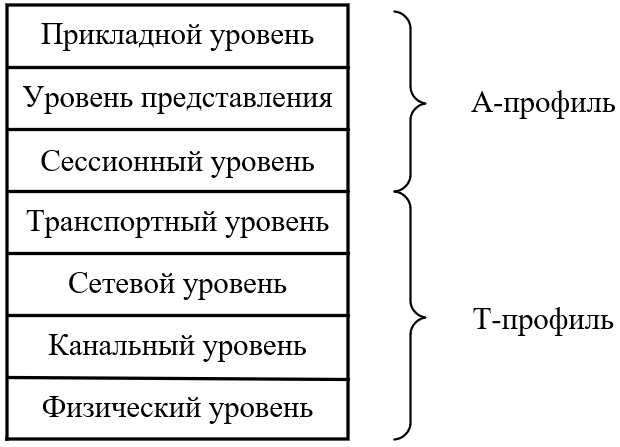
\includegraphics[width=.5\linewidth]{osiModel}
    \caption{Эталонная модель и профили OSI}
    \label{pic::domain::osi_model}
\end{figure}

В модели OSI используется два основных профиля: A-профиль -- профиль приложения
и T-профиль -- транспортный профиль. Профили сопоставлены с уровнями модели,
как изображено на рисунке~\ref{pic::domain::osi_model}. А-профиль OSI --
это набор спецификаций и соглашений, которые относятся к трем верхним уровням
эталонной модели OSI (уровень приложения, уровень представления и сессионный
уровень). Т-профиль относится к четырем нижним уровням модели
(транспортный уровень, сетевой, канальный и физический). Можно использовать
различные комбинации А- и Т-профилей, чтобы обеспечить определенные виды информации
и сервисов, подлежащих обмену. Сервисы представлены в четырех различных комбинациях
А- и Т-профилей. Они используются для следующих служб:

\begin{itemize}
    \item службы клиент/сервер, изображенные на рисунке~\ref{pic::domain::msg_types} как набор протоколов MMS;
    \item службы управления GOOSE/GSE;
    \item сервисы GSSE;
    \item сервисы синхронизации времени, изображенные на рисунке~\ref{pic::domain::msg_types} как SNTP.
\end{itemize}

\nomenclaturex{GSSE}{Generic Substation State Event}{обобщенное событие состояния подстанции}
\nomenclaturex{GSE}{Generic Substation Event}{обобщенное событие подстанции}

\subsection{Службы управления GOOSE/GSE}

Коммуникационный профиль GSE рекомендуется использовать для любой реализации,
утверждающей соответствие стандарту \iecStdRef81\ и заявляющей
о поддержке одного из сервисов \iecStdRef72, показанных
в таблице~\ref{table:domain:management_services}.

\begin{table}[ht]
    \caption{Сервисы, требующие управления коммуникационных профилей GSE и GOOSE}
    \label{table:domain:management_services}
    \begin{tabular}{| >{\raggedright}m{0.397\textwidth}
                    | >{\raggedright\arraybackslash}m{0.55\textwidth}|}
        \hline
        \centering Модель & \centering\arraybackslash Сервис \iecStdRef72 \\

        \hline
        GSE & GetReference \\

         & GetGOOSEElementNumber \\

         & SendGOOSEMessage \\

        \hline
    \end{tabular}
\end{table}

В таблице~\ref{table:domain:gse_management} показаны службы и протоколы A-профиля
для общения GOOSE и управления GSE.

\begin{table}[ht]
    \caption{Службы и протоколы A-профиля для общения GOOSE и управления GSE}
    \label{table:domain:gse_management}
    \begin{tabular}{| >{\raggedright}m{0.19\textwidth}
                    | >{\raggedright}m{0.32\textwidth}
                    | >{\raggedright\arraybackslash}m{0.41\textwidth}|}
        \hline
        \centering Уровень модели OSI &
        \centering Имя &
        \centering\arraybackslash Спецификация службы и протокола \\

        \hline
        Прикладной & Протокол GOOSE/GSE & \iecStdRef81, приложение~А \\

        \hline
        Представления & Абстрактный синтаксис & \centering\arraybackslash --- \\

        \hline
        Сессионный & & \\

        \hline
    \end{tabular}
\end{table}

T-профиль для сервисов GSE и GOOSE должен соответствовать
таблице~\ref{table:domain:t_profile_for_gse}.

На базе таблиц~\ref{table:domain:gse_management}
и~\ref{table:domain:t_profile_for_gse} были приняты соглашения о реализации служб,
представленных в таблице~\ref{table:domain:management_services}. Кодирование уровня
представления должно соответствовать основным правилам кодирования. Все PDU должны
отправляться и приниматься с использованием службы T-DATA. Адрес назначения сервиса
T-DATA для сообщения GOOSE должен содержать мультикаст MAC-адрес. Адрес источника
T-DATA для сообщения GOOSE должен содержать юникаст MAC-адрес. Адрес назначения
и адрес источника T-DATA для сообщений управления GSE должны содержать юникаст
MAC-адрес.

\nomenclaturex{PDU}{Protocol Data Unit}{блок данных протокола}

\begin{table}[ht]
    \caption{T-профиль для сервисов GSE и GOOSE}
    \label{table:domain:t_profile_for_gse}
    \begin{tabular}{| >{\raggedright}m{0.20\textwidth}
                    | >{\raggedright}m{0.35\textwidth}
                    | >{\raggedright\arraybackslash}m{0.37\textwidth}|}
        \hline
        \centering Уровень модели OSI &
        \centering Имя &
        \centering\arraybackslash Спецификация службы и протокола \\

        \hline
        Транспортный & & \\

        \hline
        Сетевой & & \\

        \hline
        \multirow{2}{0.20\textwidth}{Резервирование канала связи} & Кольцо HSR и PRP & \iec~62439-3 -- PRP или HSR \\

        \cline{2-3}
        & RSTP & \ieee~802.1D \\

        \hline
        Канальный & Маркировка приоритета / VLAN & \ieee~802.1Q \\

        \hline
        Физический (общее) & CSMA/CD & \isoIec~8802-3:2000 \\

        \hline
        % Hand fixing: https://tex.stackexchange.com/a/66599/139966
        \multirow{2}{0.20\textwidth}[-1.5em - 0.5ex]{Физический (вариант 1)}
        & 10Base-T/100Base-T
        & \isoIec~8802-3:2000 \\

        \cline{2-3}
        & Интерфейсный разъем и назначение контактов для базового интерфейса доступа ISDN
        & \isoIec~8877:1992 \\

        \hline
        % Hand fixing: https://tex.stackexchange.com/a/66599/139966
        \multirow{2}{0.20\textwidth}[-1em - 0.5ex]{Физический (вариант 2)}
        & Волоконно-оптическая система передачи 1000Base-LX
        & \isoIec~8802-2:1998, \isoIec~8802-3:2000 \\

        \cline{2-3}
        & Базовый оптоволоконный соединитель
        & \iec~60874-10-1, \iec~60874-10-2 и
        \iec~60874-10-3 \\

        \hline
    \end{tabular}
\end{table}

\nomenclaturex{PRP}{Parallel Redundancy Protocol}{протокол параллельного резервирования}
\nomenclaturex{HSR}{High-availability Seamless Redundancy}{бесперебойное резервирование с высокой доступностью}
\nomenclaturex{IEEE}{Institute of Electrical and Electronics Engineers}{институт инженеров электротехники и электроники}
\nomenclaturex{RSTP}{Rapid Spanning Tree Protocol}{ускоренный протокол STP}
\nomenclaturex{VLAN}{Virtual Local Area Network}{виртуальная локальная компьютерная сеть}
\nomenclaturex{ISDN}{Integrated Services Digital Network}{цифровая сеть интегрированных услуг}
\nomenclaturex{CSMA/CD}{Carrier Sense Multiple Access with Collision Detection}
{множественный доступ с прослушиванием несущей и обнаружением коллизий}

\subsubsection{Служба GetGoReference}

Служба GetGoReference позволяет клиенту запрашивать разрешение на получение смещений
одного или нескольких элементов. В ответе возвращается набор значений,
соответствующих запрошенным ElementOffsets. Алгоритм работы сервиса GetGoReference
изображен на рисунке~\ref{pic::domain::get_go_ref_algo}.

\begin{figure}[!htb]
    \centering
    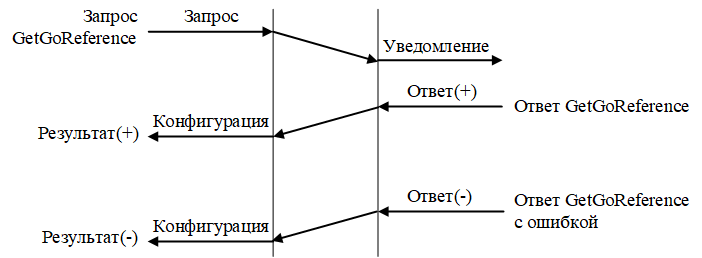
\includegraphics[width=.9\linewidth]{GetGoReference_algo}
    \caption{Алгоритм работы сервиса GetGoReference}
    \label{pic::domain::get_go_ref_algo}
\end{figure}

\nomenclaturex{MMS}{Manufacturing Message Specification}{спецификация производственного сообщения}

\begin{table}[ht]
    \caption{Параметры GetGoReference}
    \label{table:domain:get_go_ref_params}
    \begin{tabular}{| >{\raggedright}m{0.247\textwidth}
                    | >{\raggedright\arraybackslash}m{0.7\textwidth}|}
        \hline
        \centering Поле & \centering\arraybackslash Описание \\

        \hline
        Destination address & Адрес назначения должен использоваться для указания адреса, требуемого Т-профилем. \\

        \hline
        StateID & Присваиваемое клиентом значение, используемое для идентификации.
        Диапазон этого значения должен быть от $ -32767 $ до $ 32767 $. \\

        \hline
        GoCBReference & Поле типа VISIBLE\_STRING, содержащее значение,
        размер которого составляет 129 октетов. Значение должно соответствовать
        управляющему блоку GOOSE, для которого запрашивается поиск. \\

        \hline
        MemberOffsets & Это список элементов, для которых клиент запрашивает смещения. Диапазон этого значения должен быть от 0 до 512. \\

        \hline
        ConfRev & Параметр, содержащий номер версии конфигурации GoCB на момент запроса. \\

        \hline
        DatSet & Параметр, содержащий значение DataSetReference на момент запроса. \\

        \hline
        ListOfResults & Список значений запрашиваемых смещений на строки или
        соответствующий код ошибки. Отправляется с использованием сервиса T-DATA. \\

        \hline
        ErrorReason & Параметр состояния ошибки клиентского запроса. \\

        \hline
    \end{tabular}
\end{table}

Клиент присваивает идентификатор каждому запросу и включает его в качестве параметра
StateID в запрос. При получении GetGoReferenceResponse, который содержит неизвестный
StateID, клиент должен игнорировать PDU. Спецификация протокола прикладного уровня
MMS должна использоваться в качестве синтаксиса передачи для службы GetGoReference.
Сервис GetGoReference должен быть отображен, учитывая соответствие имя параметра
и синтаксиса передачи.
В таблице~\ref{table:domain:get_go_ref_params} представлено описание параметров
GetGoReference.

Все PDU управления GSE должны отправляться и приниматься с использованием службы
T-DATA.

\subsubsection{Служба GetGOOSEElementNumber}

Служба GetGOOSEElementNumber, как определено в \iecStdRef72, позволяет клиенту
запросить преобразование одной или нескольких строк в виде смещения элементов.
В ответе возвращается набор запрошенных ElementOffsets. Последовательность работы
алгоритма должна соответствовать рисунку~\ref{pic::domain::get_goose_elem_num_algo}.

\begin{figure}[ht]
    \centering
    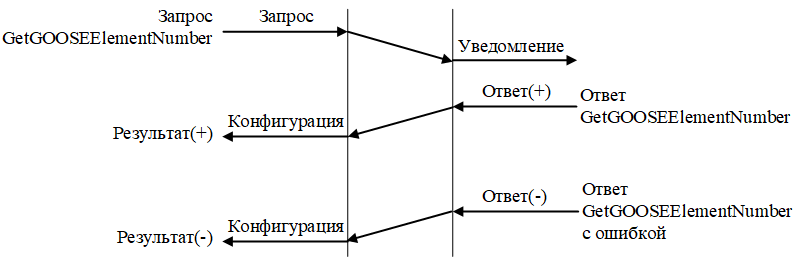
\includegraphics[width=1.\linewidth]{GetGOOSEElementNumber_algo}
    \caption{Алгоритм работы сервиса GetGOOSEElementNumber}
    \label{pic::domain::get_goose_elem_num_algo}
\end{figure}

Клиент назначает идентификатор каждому запросу, записывая его в параметр StateID
запроса. Клиент, который получает GetGOOSEElementNumberResponse, содержащий
неизвестный StateID, должен игнорировать PDU. Сервер, заявляющий о поддержке
сервиса GOOSE Management, не являющийся сервисом GetGOOSEElementNumber,
должен возвращать GseNotSupportedPDU, если был получен GetGOOSEElementNumberRequest.
Спецификация протокола прикладного уровня MMS должна использоваться в качестве
синтаксиса передачи для службы GetGOOSEElementNumber.
Сервис должен быть отображен, учитывая соответствие имя параметра
и синтаксиса передачи.

В таблице~\ref{table:domain:get_goose_elem_number_params} представлено описание
уникальных параметров GetGOOSEElementNumber. Остальные параметры соответствуют службе
GetGoReference и описаны в таблице~\ref{table:domain:get_go_ref_params}.

\begin{table}[ht]
    \caption{Параметры GetGOOSEElementNumber}
    \label{table:domain:get_goose_elem_number_params}
    \begin{tabular}{| >{\raggedright}m{0.247\textwidth}
                    | >{\raggedright\arraybackslash}m{0.7\textwidth}|}
        \hline
        \centering Поле & \centering\arraybackslash Описание \\

        \hline
        MemberReference & Список элементов, для которых клиент запрашивает смещения. Значения NULL не допускаются. \\

        \hline
        ElementNumber & Параметр содержит значение смещения для соответствующего
        запрошенного ReferenceString или причину ошибки. \\

        \hline
        T-DATA Mapping & Все PDU управления GSE должны отправляться и приниматься
        с использованием службы T-DATA T-Profile. \\

        \hline
    \end{tabular}
\end{table}

\fixTableSectionSpace

\subsubsection{Служба SendGOOSEMessage}

Модель работы GOOSE дает возможность быстрого и надежного общесистемного распределения
значений входных и выходных данных. Она использует определенную схему повторной
передачи для достижения надлежащего уровня надежности. Когда сервер GOOSE генерирует
запрос SendGOOSEMessage, текущие значения набора данных кодируются в сообщение
GOOSE и передаются через сервис T-DATA в многоадресной рассылке.
Дополнительная надежность достигается за счет повторной передачи одних
и тех же данных с постепенным увеличением SqNum и времени повторной передачи.
Алгоритм передачи данных представлен
на рисунке~\ref{pic::domain::events_transmission_time}, где:
\begin{explanationx}
    \item $ \text{Т}_0 $ -- повторная отправка в стабильных условиях (длительное отсутствие событий);
    \item $ (\text{Т}_0) $ -- повторная передача в стабильных условиях, может быть сокращена событием;
    \item $ \text{Т}_1 $ -- кратчайшее время ретрансляции после события;
    \item $ \text{Т}_2, \text{Т}_3 $ -- время повторной передачи до достижения стабильных условий.
\end{explanationx}

\begin{figure}[ht]
    \centering
    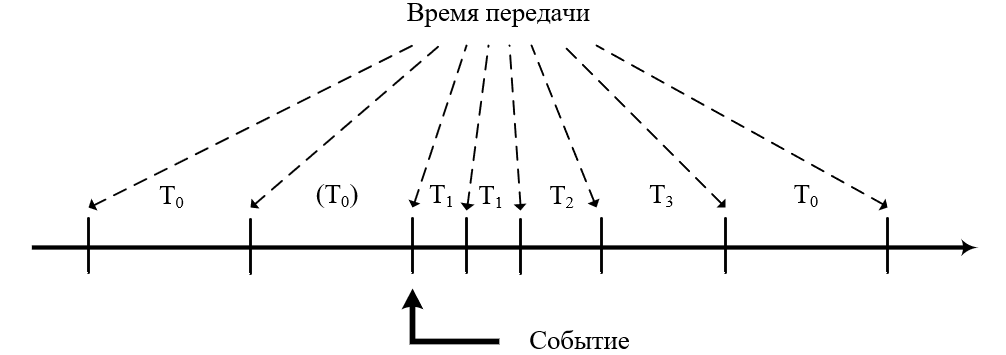
\includegraphics[width=1.\linewidth]{eventsTransmissionTime}
    \caption{Временная развертка передачи данных}
    \label{pic::domain::events_transmission_time}
\end{figure}

Каждое сообщение содержит параметр timeAllowedToLive, который сообщает получателю
максимальное время ожидания следующей повторной передачи. Если новое сообщение
не получено в течение этого интервала времени, то сообщение считается потерянным.
Интервалы, используемые сервером GOOSE, являются настраиваемым вопросом и
информируют клиентов о времени ожидания повторной отправки. Служба SendGOOSEMessage
позволяет отправлять информацию, если она была не запрошена или не подтверждена.
Алгоритм работы службы SendGOOSEMessage представлен
на рисунке~\ref{pic::domain::send_goose_msg_algo}.

\begin{figure}[ht]
    \centering
    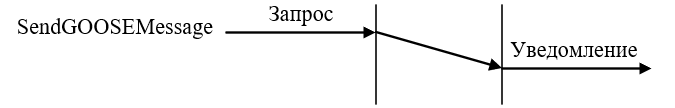
\includegraphics[width=.75\linewidth]{SendGOOSEMessage_algo}
    \caption{Алгоритм работы сервиса SendGOOSEMessage}
    \label{pic::domain::send_goose_msg_algo}
\end{figure}

Отправитель создает конечный автомат, как изображено на
рисунке~\ref{pic::domain::fsm_sender_goose}, для каждого
разрешенного GoCB, состоящий из четырех состояний:
\begin{itemize}
    \item данные не существуют;
    \item отправка данных;
    \item ожидание повторной передачи данных;
    \item повторная передача данных.
\end{itemize}

\nomenclaturex{GoCB}{GOOSE Control Block}{блок управления GOOSE}

\begin{figure}[ht]
    \centering
    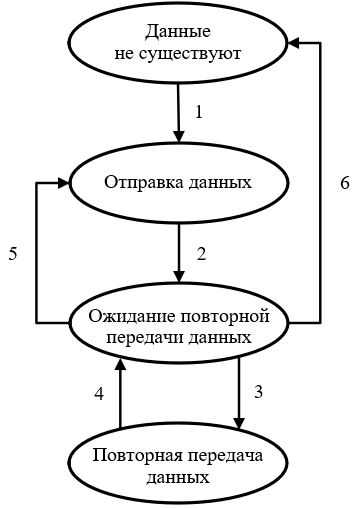
\includegraphics[width=.5\linewidth]{fsmSenderGOOSE}
    \caption{Конечный автомат отправителя для сервиса GOOSE}
    \label{pic::domain::fsm_sender_goose}
\end{figure}

Переходы состояний конечного автомата на рисунке~\ref{pic::domain::fsm_sender_goose}
происходят по следующему алгоритму:
\begin{enumerate_num}
    \item Для GoEna установлено значение TRUE.
    \item Отправитель совершает GOOSE-запрос. Таймер повторной передачи запускается
    на основе timeAllowedToLive, который установлен отправителем. Значение параметра
    SqNum устанавливается равным нулю. Предполагается, что таймер повторной передачи
    должен быть в два раза меньше параметра timeAllowedToLive.
    \item Таймер истечения повторной передачи указывает время для повторной
    передачи. SqNum увеличивается, пропуская 0 на переполнении.
    \item Повторно выполняется GOOSE-запрос. Используется следующий интервал
    повторной передачи. Запускается таймер повторной передачи. Метод выбора
    интервалов повторной передачи, как и максимальное время, допустимое между
    повторными передачами, являются локальными вопросами и устанавливаются
    на усмотрение отправителя. Допустимое время между повторными передачами должно
    составлять менее 60 секунд.
    \item При обнаружении изменения значения одного из элементов DataSet,
    StNum увеличивается, а SqNum устанавливается равным нулю.
    \item Все сообщения GOOSE и повторные передачи останавливаются, когда для GoEna
    установится значение FALSE.
\end{enumerate_num}

Получатель должен создать конечный автомат, приведенный
на рисунке~\ref{pic::domain::fsm_receiver_goose}, состоящий из трех состояний:
\begin{itemize}
    \item данные не существуют;
    \item значение данных действительно;
    \item вероятное значение данных.
\end{itemize}

\begin{figure}[ht]
    \centering
    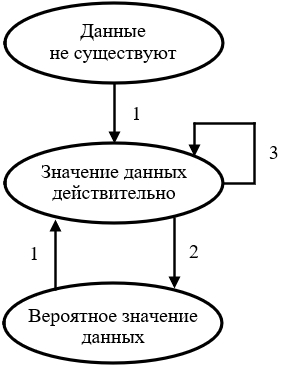
\includegraphics[width=.4\linewidth]{fsmReceiverGOOSE}
    \caption{Конечный автомат получателя для сервиса GOOSE}
    \label{pic::domain::fsm_receiver_goose}
\end{figure}

\fixTableSectionSpace

\begin{table}[ht]
    \caption{Параметры структуры DstAddress}
    \label{table:domain:dst_addr_types}
    \begin{tabular}{| >{\raggedright}m{0.137\textwidth}
                    | >{\raggedright\arraybackslash}m{0.81\textwidth}|}
        \hline
        \centering Поле & \centering\arraybackslash Описание \\

        \hline
        Addr &
        Длина составляет 6 октетов и содержит значение MAC-адреса, на который
        должно быть отправлено сообщение GOOSE. Адрес должен быть адресом Ethernet,
        для которого бит многоадресной рассылки установлен в значение TRUE. \\

        \hline
        PRIORITY & Приоритет пакета. Диапазон значений ограничен от 0 до 7. \\

        \hline
        VID & Идентификатор VLAN. Диапазон значений ограничен от 0 до 4095. \\

        \hline
        APPID & Идентификатор приложения. Алгоритм выбора значения описан
        в приложении C стандарта \iecStdRef81. \\

        \hline
    \end{tabular}
\end{table}

\nomenclaturex{MAC}{Media Access Control}{контроль за доступом к среде передачи данных}

Переходы состояний конечного автомата на
рисунке~\ref{pic::domain::fsm_receiver_goose} происходят по следующему алгоритму:
\begin{enumerate_num}
    \item Получатель принимает корректное GOOSE-сообщение и запускает таймер
    истечения срока действия timeAllowedToLive.
    \item Истекает срок действия таймера timeAllowedToLive.
    \item Получатель принимает корректное GOOSE-сообщение с новыми или
    повторяющимися данными.
\end{enumerate_num}

\subsection{Сопоставление полей протоколов GOOSE и MMS}

MMS вместе с GOOSE являются основными протоколами передачи данных стандарта
\iecStd. Он использует технологию передачи клиент-сервер, не является
коммуникационным протоколом, а только определяет сообщения, которые должны
передаваться по сети. В качестве коммуникационного протокола в MMS используется
стек TCP/IP.

Типы GOOSE должны быть сопоставлены с типами MMS~\cite{IEC61850_7_2}.
В таблице~\ref{table:domain:goose_mms_equality} приведено описание параметров,
которое используется при передаче GOOSE средствами MMS.

\begin{table}[ht]
    \caption{Параметры GOOSE при использовании MMS}
    \label{table:domain:goose_mms_equality}
    \begin{tabular}{| >{\raggedright}m{0.137\textwidth}
                    | >{\raggedright\arraybackslash}m{0.81\textwidth}|}
        \hline
        \centering Поле & \centering\arraybackslash Описание \\

        \hline
        GoEna & Должно соответствовать стандарту \iecStdRef72. \\

        \hline
        GoID & Значение по умолчанию этого атрибута должно быть ссылкой на GoCB. \\

        \hline
        DatSet &
        Должно иметь тип данных ObjectReference. Значение должно быть ограничено
        набором существующих списков NamedVariableList MMS. Значения, указывающие
        на несуществующий NamedVariableList, должны считаться ошибочными. \\

        \hline
        ConfRev &
        Беззнаковое целочисленное значение в диапазоне от 0 до $ 4294967295 $. \\

        \hline
        NdsCom &
        Этот компонент MMS представляет атрибут NdsCom стандарта \iecStdRef72. \\

        \hline
        DstAddress &
        Структурированный тип MMS, компоненты которого определены в соответствии
        с таблицей~\ref{table:domain:dst_addr_types}. \\

        \hline
        MinTime &
        Задержка отправки при изменении данных между первой отправкой и
        первым повторением. Единица измерения -- миллисекунды. \\

        \hline
        MaxTime &
        Время контроля источника в миллисекундах. В течение этого времени клиент
        должен обнаружить ошибочное сообщение от источника, если такое было. \\

        \hline
    \end{tabular}
\end{table}

\fixTableSectionSpace

% \subsection{Существующие аналоги}

% TODO: implement
